\documentclass{article}
\usepackage[utf8]{inputenc}
\usepackage{graphicx}
\title{Quantum HW2}
\author{bellenchia }
\date{February 2019}

\begin{document}

\maketitle
\section*{Normlization and Orthogonality}
\subsection*{4a}
Given a wavefuntion $\phi(x)=af(x)+bg(x)$ where $f(x)$ and $g(x)$ are orthonormal, normalizing the wavefunction yeilds;\\

%Let us assume that each of the complex constants $a$ and $b$ can be represented in the folloing forms; \\

%$a=u+iv$ and $b=p+iq$

$1=N^2{\displaystyle \int_{-\infty}^\infty}\phi^*(x)\phi(x)dx$\\

$=N^2(|a|^2<f|f>+|b|^2<g|g>+a^*b<f|g>+b^*a<g|f>)$\\

$1=N^2(|a|^2+|b|^2)$\\

$N=\frac{1}{\sqrt{|a|^2+|b|^2}}$\\

\subsection*{4b}

Now, we deal with orthogonal functions which are not normalized; such that their overlap is given by ${\displaystyle \int_{-\infty}^\infty}f^*gdx=S$

$1=N^2(|a|^2<f|f>+|b|^2<g|g>+a^*b<f|g>+b^*a<g|f>)$\\

$=N^2(|a|^2+|b|^2+(a^*b)S+(b^*a)S)$\\

$=N^2(|a|^2+|b|^2+2Re(a^*b)S)$\\

$N=\frac{1}{\sqrt{|a|^2+|b|^2+2Re(a^*b)S}}$\\

\section*{Quantum Cascade Lasers}

\subsection*{5a}

We know that the energy of the n'th state is given by $E_n=\frac{n^2\hbar^2\pi^2}{2ma^2}$\\

Thus, we have $\Delta E=E_{n+1}-E_n=\frac{(n^2+2n+1)\hbar^2\pi^2}{2ma^2}-\frac{n^2\hbar^2\pi^2}{2ma^2}=\frac{(2n+1)\hbar^2\pi^2}{2ma^2}$\\

Where $m=0.07m_e$, $m_e$ being the mass of an electron\\

\subsection*{5b}

Using the photon energy relation $E_\gamma=\frac{hc}{\lambda}$ and setting it equal to our energy difference, we can solve for a, the necessary width of the layer\\

$\frac{(2n+1)\hbar^2\pi^2}{2ma^2}=\frac{hc}{\lambda}\Rightarrow a=\sqrt{\frac{3\pi^2\hbar^2\lambda}{2mhc}}$\\

Plugging in all our values, we get $a=1.08*10^{-8}$\\

\section*{Particle \textit{Moving} in a Box}

\subsection*{6a}

Given the wavefunction at $t=0$, $\Psi(x,0)=\frac{1}{\sqrt{L}}(sin\frac{\pi x}{L}+\sin\frac{2\pi x}{L})$\\

We know that the wave function is a sum of our spatial components with their corresponding time dependencies;\\

$\Psi(x,t)=\sum_{n=1}^2\phi(x)e^{-iE_nt/\hbar}$ Where $E_n=\frac{n^2\hbar^2\pi^2}{2ma^2}$\\

$\Rightarrow\Phi(x,t)=\frac{1}{\sqrt{L}}(sin\frac{\pi x}{L}e^{-i\hbar\pi^2/2ma^2}+\sin\frac{2\pi x}{L}e^{-2i\hbar\pi^2/ma^2})$\\

\subsection*{6b}
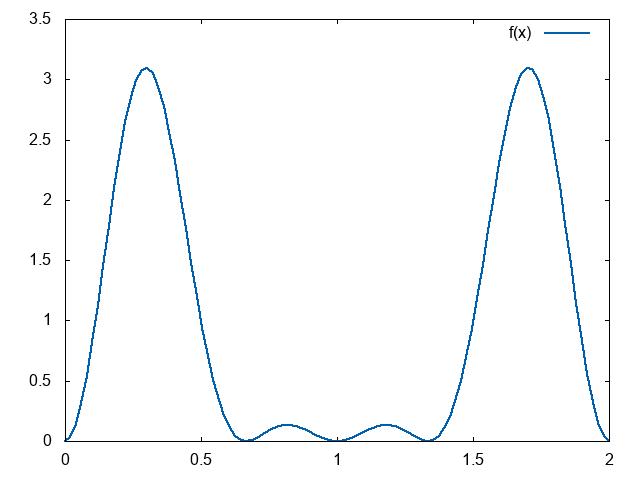
\includegraphics[width=\textwidth]{plot1.png}
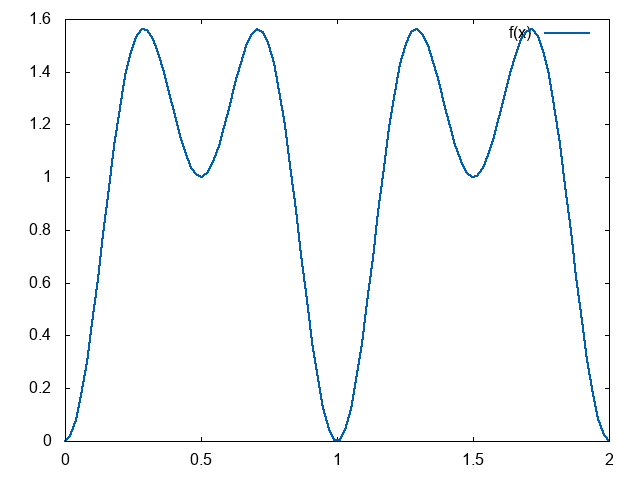
\includegraphics[width=\textwidth]{plot2.png}
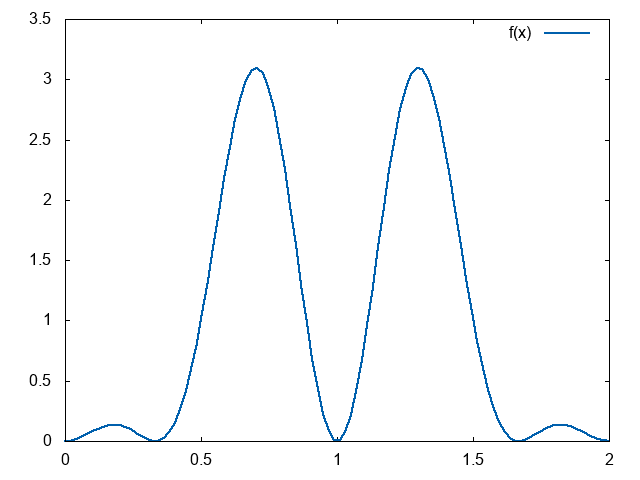
\includegraphics[width=\textwidth]{plot3.png}
\subsection*{6c}

The total energy is independant of time, and can be calculated by the following\\

$<\hat{H}>=\sum|c_n|^2E_n=\frac{1}{L}(\frac{\hbar^2\pi^2}{2ma^2}+\frac{4\hbar^2\pi^2}{2ma^2})=\frac{5\hbar^2\pi^2}{2mL^3}$\\

\subsection*{6d}

$<x>(t)={\displaystyle\int_0^L}\Psi^*x\Psi dx$\\

$=\frac{1}{L}((sin\frac{\pi x}{L}e^{i\hbar\pi^2/2ma^2}+sin\frac{2\pi x}{L}e^{2i\hbar\pi^2/ma^2}))x((sin\frac{\pi x}{L}e^{-i\hbar\pi^2/2ma^2}+sin\frac{2\pi x}{L}e^{-2i\hbar\pi^2/ma^2}))$\\

$={\displaystyle\int_0^L}xsin^2\frac{\pi x}{L}+xsin^2\frac{2\pi x}{L}+2xsin\frac{\pi x}{L}sin\frac{2\pi x}{L}cos(\frac{E_2-E_1}{\hbar}t)$\\

$=\frac{1}{L}(\frac{L^2}{4}+\frac{L^2}{4}-\frac{16L^2}{9\pi^2}cos(\frac{E_2-E_1}{\hbar}t))=\frac{L}{2}-\frac{16L}{9\pi^2}cos(\frac{E_2-E_1}{\hbar}t)$\\

\section*{Free Particles, Wave Packets, and Quantum Diffusion}

\subsection*{7a}

Given the wavefunction $\Psi(x,t)=Ae^{i(k_0x-\omega t)}$ we plug into 1-dimensional TDSE;\\

$\frac{-\hbar^2}{2m}\frac{d^2}{dx^2}(Ae^{i(k_0x-\omega t)})=i\hbar\frac{d}{dt}(Ae^{i(k_0x-\omega t)})\Rightarrow \omega=\frac{k_0^2\hbar^2}{2m}$\\

Plugging this back into the equation and writing as a seperable solution;\\

$\Psi(x,t)=Ae^{ik_0x}e^{-i\hbar k_0^2t/2m}$\\

Since our temporal component is of the form $\phi(t)=e^{-iEt/\hbar}$ we write;\\

$\frac{E}{\hbar}=\frac{\hbar k_0^2}{2m}\Rightarrow E=\frac{\hbar^2k_0^2}{2m}$\\

The speed of the wave is $\frac{\hbar k_0}{2m}$

\subsection*{7b}

Now, substitution into the 1D wave equation $\frac{d^2}{dt^2}\Psi=c^2\frac{d^2}{dx^2}\Psi$ we get \\

$(-i\omega)(-i\omega)Ae^{i(k_0x-\omega t)}=c^2(ik_0)(ik_0)Ae^{i(k_0x-\omega t)}\Rightarrow\omega=\sqrt{c^2k_0^2}$\\

The speed of this wave is $c$, analogous to lightspeed\\

\subsection*{7c}

Given $\Psi(x,t)=\sqrt{\frac{t_0}{t}}e^{-x^2/4Dt}$, we substitute into $\frac{d\Psi}{dt}=D\frac{d^2\Psi}{dx^2}$\\

$\frac{d\Psi}{dt}=\sqrt{t_0}(\frac{-1}{2}t^{-1/2}e^{-x^2/4Dt}+\frac{x^2}{4Dt^2}e^{-x^2/4Dt})=\sqrt{\frac{t_0}{t}}e^{-x^2/4Dt}(\frac{x^2-4Dt}{4Dt^2})$\\

$\frac{d^2\Psi}{dx^2}=\frac{d}{dx}[\sqrt{\frac{t_0}{t}}\frac{2x}{4Dt}e^{-x^2/4Dt}]=\sqrt{\frac{t_0}{t}}\frac{2}{4Dt}e^{-x^2/4Dt}(\frac{2x^2}{4Dt}-1)$\\

\end{document}
